\section{Πλοήγηση Οχήματος και Κάλυψη του Χώρου}
\label{section:navigation_and_coverage}

Σημαντικό μέρος της εργασίας αποτελεί η δημιουργία του συστήματος πλοήγησης του ρομποτικού οχήματος στον χώρο και η συνεχής καταγραφή των περιοχών που καλύπτουν οι κεραίες που φέρει. Τα δύο αυτά συστήματα είναι η βάση όλης της μελέτης της παρούσας εργασίας. Η υλοποίηση τους παρουσιάζεται στη συνέχεια. 


\subsection{Υλοποίηση Πλοήγησης}
\label{section:navigation_implementation}

Η πλοήγηση του ρομποτικού οχήματος στον εικονικό κόσμο επιτυγχάνεται με τη χρήση του Navigation Stack \ref{section:navigation_stack}. Αυτό διευκολύνει σημαντικά τη διαδικασία, καθώς απαιτεί μόνο τις τρεις μεταβλητές του σημείου στόχου, δηλαδή τη θέση και τον προσανατολισμό του. Το stack παράγει την τροχιά που χρειάζεται να ακολουθήσει το όχημα για να βρεθεί στον ζητούμενο στόχο και του δίνει τις κατάλληλες εντολές ταχύτητας. 

Η ανάπτυξη του συστήματος βασίστηκε στο \cite{navStack} και παρουσιάζεται στους επόμενους δύο αλγορίθμους. Ο πρώτος \ref{alg:go_to_goal} διαβάζει τη θέση και τον προσανατολισμό του σημείου στόχου, τον μετασχηματίζει στην κατάλληλη μορφή, δημιουργεί το μήνυμα $goal$ και το στέλνει στο stack περιμένοντας την επιτυχή εκτέλεση του. Ο δεύτερος \ref{alg:navigation} αποτελεί τον βασικό αλγόριθμο της διαδικασίας και υπολογίζει το τρέχον δωμάτιο διαβάζοντας τη θέση του οχήματος στο OGM και για κάθε δωμάτιο σύμφωνα με την αλληλουχία που έχει υπολογιστεί ανακαλεί τα σημεία στόχους του. Κάθε σημείο διαχωρίζεται σε θέση και προσανατολισμό και καλείται η συνάρτηση \emph{goToGoal}. Τέλος, μόλις το όχημα προσεγγίσει τον στόχο παραμένει εκεί για 0.1 δευτερόλεπτα, για την καλύτερη κάλυψη του χώρου, πριν συνεχίσει για το επόμενο σημείο.


\begin{algorithm}[H]
\caption{Go To Goal}
\label{alg:go_to_goal}
\begin{algorithmic}[1]
    \Function{goToGoal}{target, yaw}
        \State Set $resolution$ equal to map's resolution
        \State Set $origin$ equal to map's origin
        \State $move\_base\_client.wait\_for\_server()$
        \State $goal = MoveBaseGoal()$
        \State $goal.target\_pose.header.frame\_id = 'map'$
        \State $goal.target\_pose.header.stamp = rospy.Time.now()$
        \State $goal.target\_pose.pose.position.x = target[0]*resolution + origin['x']$
        \State $goal.target\_pose.pose.position.y = target[1]*resolution + origin['y']$
        \State $quaternion = tf.transformations.quaternion\_from\_euler(0, 0, yaw)$
        \State $goal.target\_pose.pose.orientation.x = quaternion[0]$
        \State $goal.target\_pose.pose.orientation.y = quaternion[1]$
        \State $goal.target\_pose.pose.orientation.z = quaternion[2]$
        \State $goal.target\_pose.pose.orientation.w = quaternion[3]$
        \State $move\_base\_client.send\_goal(goal)$
        \State $wait = move\_base\_client.wait\_for\_result()$
        \State \Return $move\_base\_client.get\_result()$
\end{algorithmic}
\end{algorithm}



\begin{algorithm}[H]
\caption{Navigation}
\label{alg:navigation}
\begin{algorithmic}[1]
    \Function{navigation}{sequence, rooms}
    \State Read robot's current pose
    \State Compute current room
    \For{each $room$ in $sequence$ starting from current}
        \For{each $pose$ in $room$}
            \State $result = goToGoal(pose['position'], pose['yaw'])$
            \State $rospy.sleep(0.1)$
        \EndFor
    \EndFor
    \State \Return 
\end{algorithmic}
\end{algorithm}

\subsection{Υλοποίηση Κάλυψης Χώρου}
\label{section:coverage_implementation}

Η δεύτερη υλοποίηση αφορά την συνεχή καταγραφή της κάλυψης του χώρου. Το σύστημα αυτό λειτουργεί παράλληλα με όλα τα υπόλοιπα χωρίς να τα επηρεάζει ως μια ξεχωριστή διεργασία. 

Το όχημα φέρει ένα σύνολο αισθητήρων με χαρακτηριστικά τα οποία ορίζονται στην αρχή της διαδικασίας και είναι το μήκος της ακτίνας κάλυψης, το γωνιακό εύρος κάλυψης FOV και η γωνία τοποθέτησης της κεραίας ως προς το εμπρός μέρος του οχήματος. Το σχήμα του πεδίου κάλυψης είναι ουσιαστικά ένα τμήμα ενός κύκλου, όπως φαίνεται και στις δύο εικόνες \ref{fig:sensor_field_example}, όπου με μπλε χρώμα είναι σκιασμένες οι περιοχές κάλυψης. Στην πρώτη το όχημα φέρει μια κεραία με ευρεία γωνία κάλυψης ενώ στην δεύτερη φέρει δύο, μικρότερου εύρους, τοποθετημένες συμμετρικά στις δύο πλευρές του.

\begin{figure}[!htb]
    \centering
    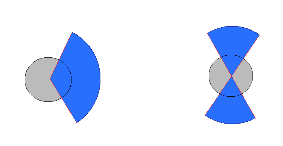
\includegraphics[width=0.4\textwidth]{./images/chapter5/sensor_field_example.png}
    \caption{Παράδειγμα Κάλυψης Αισθητήρων}
    \label{fig:sensor_field_example}
\end{figure}

Στην διπλωματική αυτή εργασία γίνεται μελέτη τριών διαφορετικών στοιχείων της κάλυψης του χώρου κατά την πλοήγηση του οχήματος. Αυτά είναι τα εξής:
\begin{itemize}
    \setlength\itemsep{-0.2em}
    \item Κάλυψη του χώρου 
    \item Πλήθος διαφορετικών σαρώσεων κάθε σημείου
    \item Γωνία σάρωσης κάθε σημείου
\end{itemize}
Συγκεκριμένα, το πρώτο αναφέρεται στην vanilla κάλυψη του χώρου, δηλαδή εάν οι αισθητήρες έχουν σαρώσει κάθε σημείο ξεχωριστά. Το δεύτερο αναφέρεται στον αριθμό σαρώσεων κάθε σημείου. Όσες περισσότερες φορές δει ο αισθητήρας κάποιο σημείο, τόσο πιο σίγουρος θα είναι για την ύπαρξη ή μη ετικετών RFID στο σημείο αυτό. Το τελευταίο αναφέρεται στην γωνία υπό την οποία σάρωσε ο αισθητήρας ένα σημείο. Στην ιδανική περίπτωση στόχος είναι να σαρωθεί ένα εμπόδιο τόσο από το θετικό μισό τόξο του αισθητήρα, όσο και από το αρνητικό. Με τον τρόπο αυτό η ετικέτα RFID θα αναγνωσθεί από διαφορετική φάση, κάτι που οδηγεί σε αποτελεσματικότερο εντοπισμό της θέσης της. Ο εντοπισμός των ετικετών εξαρτάται κυρίως από την ισχύ του λαμβανόμενου σήματος, την απόσταση του από την κεραία και την φάση του σήματος. Συνεπώς, η ακρίβεια αυξάνεται σημαντικά χρησιμοποιώντας πληθώρα διαφορετικών μετρήσεων, όπως αναφέρουν και ο Nikitin κ.ά. \cite{rfidNikitin} και ο Hekimian-Williams κ.ά. \cite{rfidHekimian}.

Η πρόταση αυτή γίνεται αντιληπτή στο σχήμα \ref{fig:different_angle_cover_example}, όπου ένα σημείου του τοίχου σαρώνεται από τον αισθητήρα δύο φορές, κάθε μία από διαφορετικό μισό του FOV του αισθητήρα. Θεωρώντας την κεντρική ακτίνα του FOV ως τις 0 μοίρες το τόξο κάλυψης χωρίζεται σε δύο ίσα τμήματα, το αριστερό (αρνητικό) και το δεξιό (θετικό). Βέβαια, αυτή η μέτρηση αφορά σημεία τα οποία έχουν σαρωθεί τουλάχιστον μία φορά από τους αισθητήρες. Έτσι, μπορεί να χρησιμοποιηθεί η παρακάτω μετρική:

\[coverage\_angles = \frac{\abs{left - right}}{left + right}\]
Όσο πιο ομοιόμορφη είναι η κατανομή σαρώσεων μεταξύ των δύο τμημάτων και όσο περισσότερες είναι οι σαρώσεις συνολικά, τόσο η μετρική θα προσεγγίζει το μηδέν, αλλιώς θα προσεγγίζει τη μονάδα.

\begin{figure}[!htb]
    \centering
    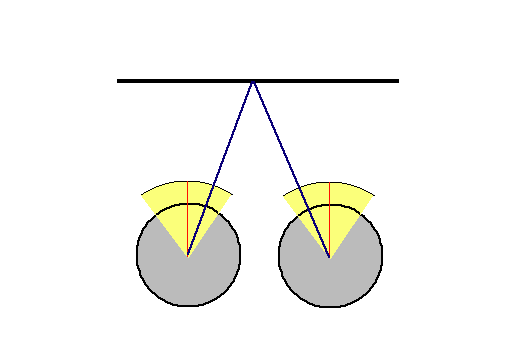
\includegraphics[width=0.7\textwidth]{./images/chapter5/different_angle_cover_example.png}
    \caption{Παράδειγμα Κάλυψης Σημείου υπό Διαφορετικών Γωνιών}
    \label{fig:different_angle_cover_example}
\end{figure}

Συμπερασματικά, η κάθε κάλυψη μπορεί να ποσοτικοποιηθεί στις παρακάτω πέντε μετρικές, οι οποίες και χρησιμοποιήθηκαν σε όλα τα πειράματα κάλυψης χώρου.
\begin{itemize}
    \setlength\itemsep{-0.2em}
    \item Ποσοστό συνολικής κάλυψης των εμποδίων του χώρου
    \item Μέση τιμή πλήθους σαρώσεων κάθε σημείου
    \item Διακύμανση πλήθους σαρώσεων κάθε σημείου
    \item Μέση τιμή μετρικής γωνίας σάρωσης κάθε σημείου που έχει σαρωθεί
    \item Διακύμανση μετρικής γωνίας σάρωσης κάθε σημείου που έχει σαρωθεί
\end{itemize}


Η υλοποίηση του συστήματος αυτού περιλαμβάνει δύο συναρτήσεις. Η πρώτη \ref{alg:circular_ray_cast_coverage} είναι αυτή που βρίσκει τα σημεία του OGM που καλύπτονται κάθε φορά από έναν αισθητήρα του ρομποτικού οχήματος. Για δεδομένα χαρακτηριστικά αισθητήρα και πόζα του οχήματος υπολογίζονται τα σημεία με τη χρήση του brushfire αλγορίθμου και της ray casting τεχνικής. Συγκεκριμένα, δημιουργείται μια ακτίνα από την κεραία προς τα έξω, πάνω στην οποία εκτελείται ο αλγόριθμος brushfire μέχρι να συναντήσει εμπόδιο ή να ξεπεράσει την ακτίνα κάλυψης του αισθητήρα. Όλα τα ελεύθερα σημεία στα οποία διαδίδεται ο brushfire είναι αυτά που καλύπτει ο αισθητήρας. Η διαδικασία αυτή εκτελείται επαναληπτικά για όλες τις ακτίνες μέσα στο FOV του αισθητήρα με πολύ μικρό βήμα, ίσο με $0.5$ μοίρες. Επίσης, υπάρχει η επιλογή μέσω της μεταβλητής εισόδου $return\_obstacles$ ο αλγόριθμος να επιστρέψει είτε τα σημεία του ελεύθερου χώρου είτε το σύνολο των εμποδίων που σαρώνονται. 

Η μέθοδος αυτή φέρει σημαντικά πλεονεκτήματα. Συγκεκριμένα, με τη χρήση του brushfire, η εξάπλωση περιορίζεται αποκλειστικά στον γύρω ελεύθερο χώρο και δεν σαρώνονται τα σημεία εμποδίων. Πράγματι, η εξάπλωση σταματάει για κάθε ακτίνα μόλις εντοπιστεί εμπόδιο και παραμένει στο ίδιο δωμάτιο. Συνεπώς, δεν σαρώνονται σημεία πίσω από τοίχους, κάτι που ρεαλιστικά οι αισθητήρες αδυνατούν να κάνουν. Επιπλέον, η χρήση της ray casting τεχνικής προσομοιώνει την πραγματική λειτουργία του αισθητήρα, καθώς αυτός σαρώνει σε συγκεκριμένο πεδίο ενός κύκλου το οποίο μπορεί να προσεγγιστεί ικανοποιητικά χρησιμοποιώντας ένα μεγάλο πλήθος ακτίνων.

Ο \autoref{alg:update_cover} συντονίζει τη διαδικασία κάλυψης. Διαβάζει, αρχικά, την τρέχουσα θέση του οχήματος και ελέγχει εαν αυτό έχει κινηθεί, συγκρίνοντας την με την προηγούμενη μέτρηση. Αυτός ο έλεγχος γίνεται για εξοικονόμηση υπολογιστικής ισχύος, καθώς όταν το όχημα παραμένει ακίνητο οι αισθητήρες εντοπίζουν τα ίδια σήματα. Εαν το ρομπότ έχει κινηθεί ως προς οποιαδήποτε από τις τρεις μεταβλητές υπολογίζονται τα σημεία που καλύπτει το σύνολο των αισθητήρων του. Μετά, για κάθε σημείο ανανεώνεται η τιμή κάλυψης του στον πίνακα $coverage$, ο οποίος έχει διαστάσεις ίσες με το OGM του χώρου και αποθηκεύει την κάλυψη ή όχι του κάθε διακριτού σημείου με τιμές $100$ και $0$, αντίστοιχα. Επίσης, ανανεώνεται η τιμή πλήθους σαρώσεων στον $coverage\_number$, αλλά και του πλήθους σαρώσεων κάθε τμήματος γωνιών στον $coverage\_angles$, έναν τρισδιάστατο πίνακα με τρίτη διάσταση ίση με 2. 

Ένα παράδειγμα του πίνακα $coverage$ παρουσιάζεται στο \ref{fig:coverage_ogm_example}, όπου φαίνεται το OGM του περιβάλλοντος και με σκούρο γκρι χρώμα είναι σημειωμένα όλα τα σημεία τα οποία καλύφθηκαν από τους αισθητήρες κατά την πλοήγηση του στον χώρο. 


\begin{figure}[!htb]
    \centering
    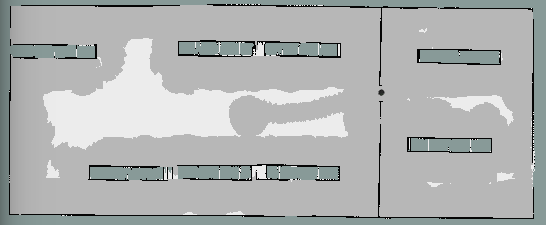
\includegraphics[width=0.8\textwidth]{./images/chapter5/warehouse_4_wall_follow_a_priori_coverage_085_weights_1_2_real.png}
    \caption{Παράδειγμα Πεδίου Κάλυψης}
    \label{fig:coverage_ogm_example}
\end{figure}

\begin{algorithm}[H]
\caption{Circular Ray Cast Coverage}
\label{alg:circular_ray_cast_coverage}
\begin{algorithmic}[1]
    \Function{circularRayCastCoverage}{start, ogm, cover\_range, fov, theta, direction, return\_obstacles = False}
    \State $brushfire = numpy.zeros(ogm.shape, np.dtype('int32'))$
    \State $brushfire[ogm > 49] = 1$
    \State $brushfire[ogm == -1] = -1$
    \State $brushfire[start] = 2$
    \State $th = -fov/2$
    \While{$th <= fov/2$}
        \State $angle = (th + direction + theta) *  $ π $/ 180.0;$
        \State $step = 2$, $iters = 1$
        \While{$iters <= cover\_length$}
            \State $xx = (int) round(start[0] + cos(angle) * iters)$
            \State $yy = (int) round(start[1] + sin(angle) * iters)$
            \If{$brushfire[xx][yy] == 0$}
                \State $brushfire[xx][yy] = step$
                \State $step++$
            \ElsIf{$brushfire[xx][yy] == 1$}
                \State $brushfire[xx][yy] = -2$
                \State break
            \ElsIf{$brushfire[xx][yy] < 0$}
                \State break
            \EndIf
            \State $iters++$
        \EndWhile
        \State $th += 0.5$
    \EndWhile
    \If{return\_obstacles}
        \State $indexes = zip(*numpy.where(brushfire == -2))$
    \Else
        \State $indexes = zip(*numpy.where(brushfire > 1))$
    \EndIf
    \State \Return $indexes$
\end{algorithmic}
\end{algorithm}


\begin{algorithm}[H]
\caption{Update Cover}
\label{alg:update_cover}
\begin{algorithmic}[1]
    \Function{updateCover}{previous\_robot\_pose, ogm, coverage, coverage\_number, coverage\_angles, resolution,  sensor\_range, sensor\_fov, sensor\_direction}
    \State Read robot's pose $xx$, $yy$, $th$
    \State Check if robot has been moved from previous pose 
    \If{robot moved}
        \For{each sensor $s$}
            \State $cover\_length = int(sensor\_range[s] / resolution)$
            \State $indexes = circularRayCastCoverage((xx,yy), ogm, cover\_length,$\par
            \hskip\algorithmicindent $sensor\_fov[s], th, sensor\_direction[s])$
            \For{$x$, $y$ in $indexes$}
                \State $coverage[x, y] = 100$
                \State $coverage\_number[x, y] += 1$
                \State $angle = th + sensor\_direction[s] + math.degrees(math.atan2(yy-y,xx-x))$
                \If{$angle < 0$}
                    \State $coverage\_angles[x, y][0] += 1$
                \Else
                    \State $coverage\_angles[x, y][1] += 1$
                \EndIf
            \EndFor
        \EndFor
    \EndIf
    \State  Update $previous\_robot\_pose$ with current pose
    \State \Return $coverage$, $coverage\_number$, $coverage\_angles$, $previous\_robot\_pose$
\end{algorithmic}
\end{algorithm}

